% !TEX root = ../main.tex

\chapter{Especificações do produto}

\section{Funcionalidades e interações suportadas}
Como demonstrado na figura \ref{fig:interface_current}, esta plataforma é uma aplicação simples que permite aos seus 
utilizadores obterem a qualidade do ar para um determinado lugar, indicando as coordenadas. Permite não só
saber a qualidade atual, mas também a passada e futura. As métricas que ela disponibiliza são a \textbf{data 
referente à qualidade do ar}, o \textbf{valor escalar e textual da qualidade do ar}, o \textbf{poluente 
dominante} e a \textbf{concentração e valor escalar e textual da qualidade do ar referente a cada um dos
poluentes principais}.

\begin{figure}[h]
   \centering
   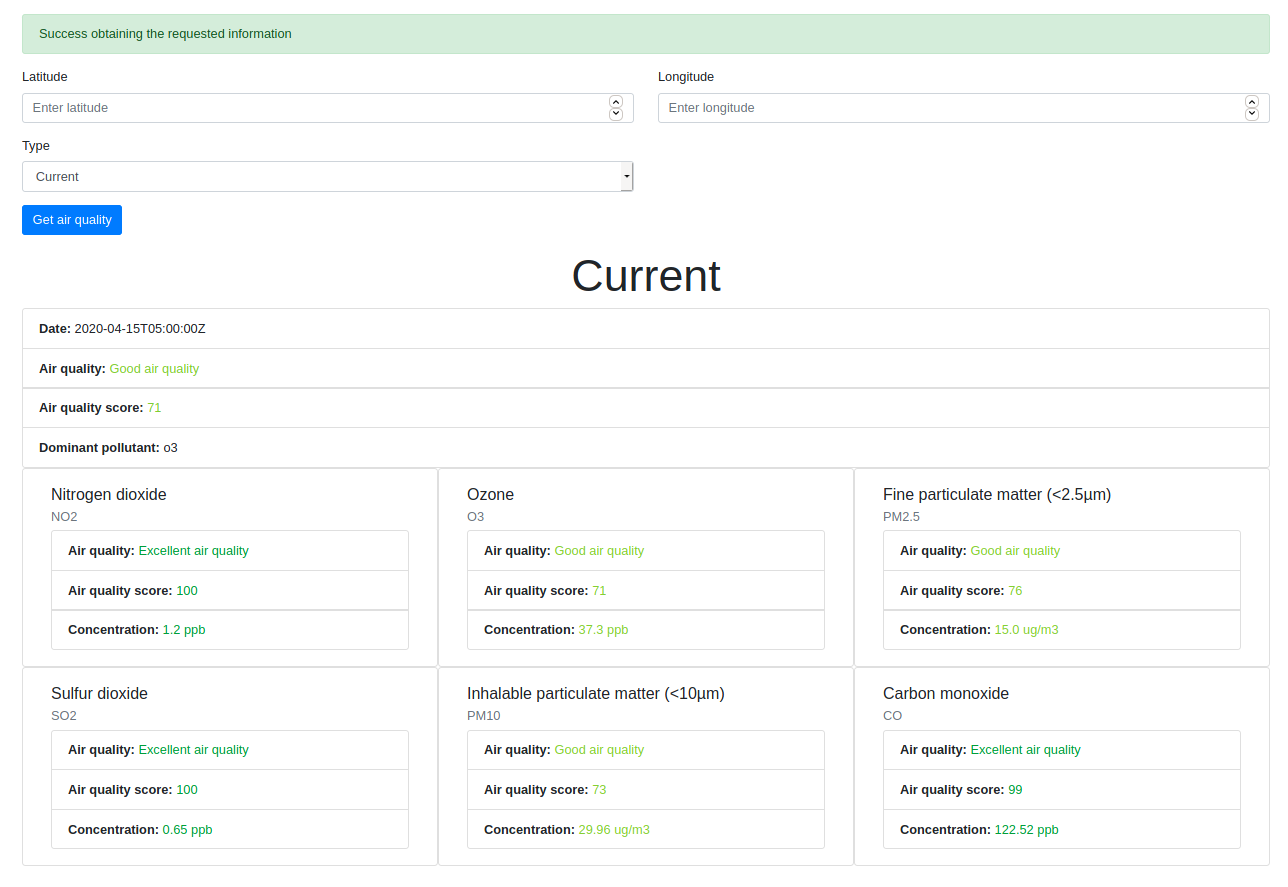
\includegraphics[width=0.90\textwidth]{images/interface_current}
   \caption{\textit{Print} da interface quando feito um pedido da qualidade do ar atual.}
   \label{fig:interface_current}
\end{figure}

Os possíveis utilizadores e cenários da plataforma criada são:

\begin{itemize}
   \item \textbf{População de risco}: dado o estado debilitado desta fração de população, é do interesse 
de algumas saber a qualidade do ar que respiram, principalmente as que possuem problemas respiratórios, 
de forma a melhor controlarem o seu estado de saúde. Desta forma, uma pessoa nestas condições poderá dirigir-se
à interface desta aplicação, introduzir as coordenadas do local onde se encontra ou se vai encontrar nos próximos
tempos, selecionar a obtenção de dados sobre o estado atual (\textit{Type Current}) ou sobre o estado previsto no 
futuro (\textit{Type Forecast}, selecionando também o número de horas seguintes sobre as quais pretende obter os 
dados) e, sendo assim, obter o estado da qualidade do ar atual ou nas horas seguintes, respetivamente.
   \item \textbf{Estudiosos}: profissionais que tenham interesse em estudar a qualidade de ar de acordo com 
o local, como por exemplo o estudo da evolução num determinado lugar. Sendo assim, um utilizador deste tipo
pode dirigir-se à página \textit{web}, selecionar um determinado lugar introduzindo as correspondentes coordenadas,
se pretende os dados de previsões passadas (\textit{Type History}) ou futuras (\textit{Type Forecast}) e o 
número de horas de dados deste o momento atual pretende obter. A partir dos resultados obtidos, poderá copiar
cada um deles e fazer o correspondente estudo.
\end{itemize}


\section{Arquitetura do sistema}
O \textit{back-end} do projeto foi feito usando \textit{java} com \textit{Maven} e \textit{Spring Boot}.
Quanto á arquitetura, é apresentado um diagrama de classes simples da mesma na figura 
\ref{fig:simple_diagram} (este diagrama de classes apenas contém as classes criadas e as relações entre elas,
sendo que os detalhes de cada uma se encontrarão definidos em diagramas expostos em subsecções seguintes, 
de forma a que este não fique demasiado confuso). Estas classes foram organizadas, de acordo com 
a sua complexidade em 4 \textit{packages}: \textbf{controller}, \textbf{model}, \textbf{serializers} e 
\textbf{service}. Nas subsecções seguintes

\begin{figure}[h]
   \centering
   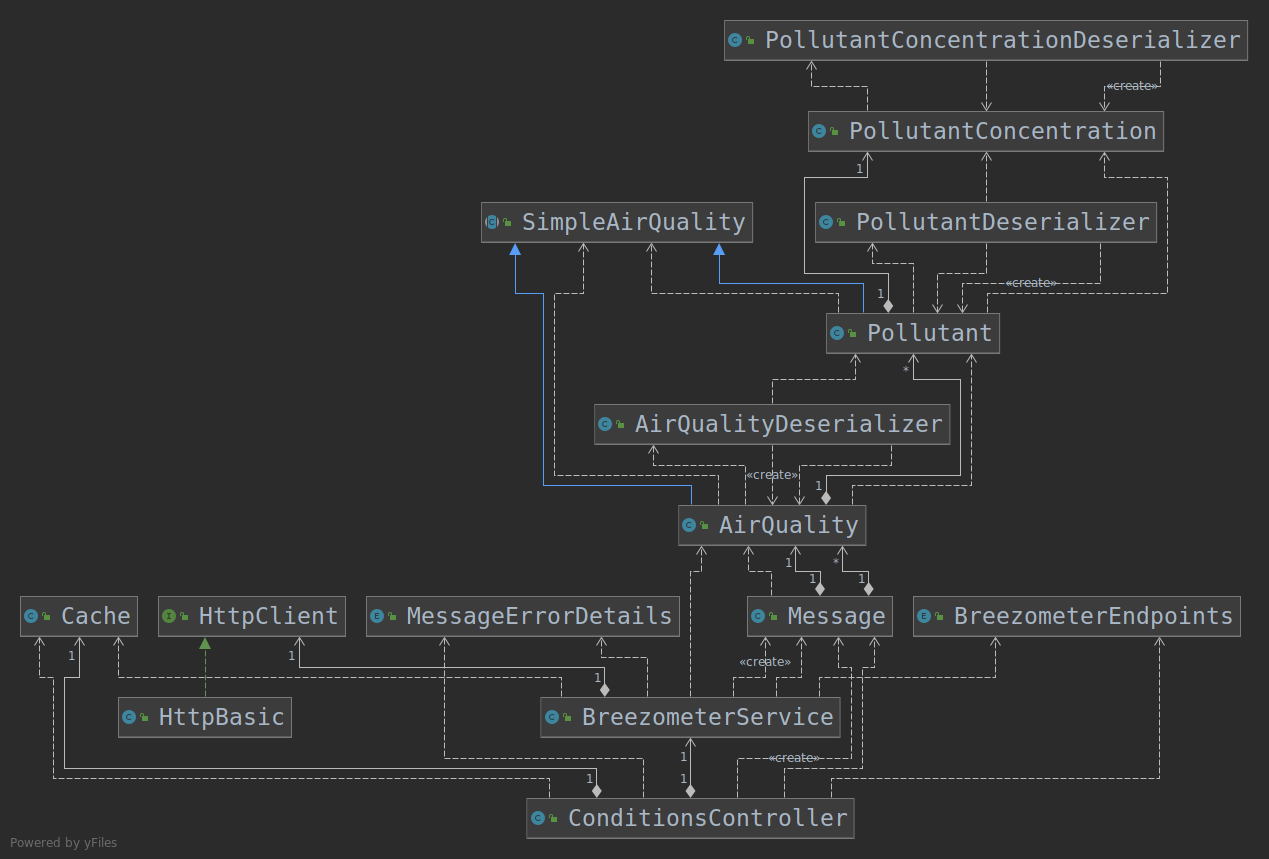
\includegraphics[width=0.90\textwidth]{images/simple_diagram}
   \caption{Diagrama de classes simples do projeto.}
   \label{fig:simple_diagram}
\end{figure}


\subsection{Package controller}
Este \textit{package} é constituído apenas por uma classe, \textbf{\textit{ConditionsController}}, que é
a responsável por lidar com as ligações feitas à \textit{API} criada. Desta forma, nesta classes são
definidos os \textit{endpoints} do nosso serviço e é definida a forma como cada \textit{request} vai ser
consumido no \textit{back-end}. Na figura \ref{fig:controller_diagram} é possível encontrar o esquema da
classe descrita.

\begin{figure}[h]
   \centering
   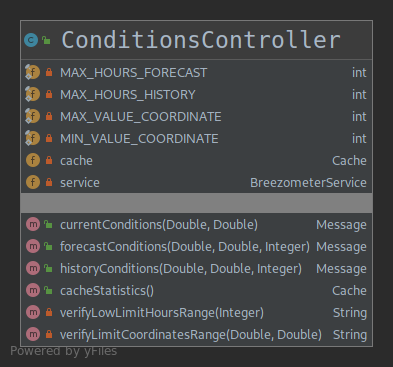
\includegraphics[width=0.40\textwidth]{images/controller_diagram}
   \caption{Diagrama das classes do \textit{package \textbf{controller}}.}
   \label{fig:controller_diagram}
\end{figure}


\subsection{Package model}
Todas as entidades usadas pelo nosso servido são representadas pelas classes deste \textit{package}. Desta forma, nela estão incluídas as classes:
\begin{itemize}
   \item \textbf{Que representam os dados da qualidade do ar}: 
      \begin{itemize}
         \item \textbf{\textit{AirQuality}}: representa a qualidade do ar referente a um determinado momento. Sendo assim, para além dos objetos desta classe possuírem informações básicas sobre a qualidade do ar, contêm também uma lista de poluentes (classe \textbf{\textit{Pollutant}}) que se encontram no ar no instante que esse objeto retrata.
         \item \textbf{\textit{Pollutant}}: classe que contém informações sobre um determinado poluente, como a forma como o respetivo poluente afeta a qualidade do ar e a concentração deste num determinado momento (classe \textbf{\textit{PollutantConcentration}}).
         \item \textbf{\textit{PollutantConcentration}}: classe que representa a informação da concentração dum poluente.
      \end{itemize}
   \item \textbf{Que modelam o sistema de cache}:
      \begin{itemize}
         \item \textbf{\textit{Cache}}: classe que permite criar objetos que simulam um sistema de cache simples e com as respetivas métricas (como o tamanho da cache ou o número de \textit{hits} e \textit{misses}). Por \textit{default}, os objetos de cache criados possuem um tamanho máximo determinado pelo valor da constante \textit{DEFAULT\_MAX\_SIZE}, sendo que quando o tamanho dela chega a esse tamanho máximo, os dados mais antigos são excluídos.
         \item \textbf{\textit{ParametersEncapsulation}}: classe que permite fazer o encapsulamento dos parâmetros sobre os quais se pretende armazenar a resposta dada pelo serviço externo na cache, isto é, quando é feito um pedido da qualidade do ar ao serviço externo, com uma determinada latitude, longidute, tipo de resposta (\textit{current}, \textit{history} ou \textit{forecast}) e possivelmente um número de horas, o resultado deste pedido pode ser armazenado na cache com um identificador representado pelo encapsulamento destes parâmetros.
      \end{itemize}
   \item \textbf{Ligadas às mensagens criadas pelo serviço}:
      \begin{itemize}
         \item \textbf{\textit{Message}}: classe que permite encapsular a resposta dada pela \textit{API} a um determinado pedido feito. Desta forma, ela tem um campo de sucesso, um de detalhes (para mensagens de sucesso ou erro), um da qualidade de ar (quando é feito um pedido da atual) e de uma lista de várias medições da qualidade do ar (quando é feito um pedido sobre os dados do passado ou futuro).
         \item \textbf{\textit{MessageErrorDetails}}: enumerável com as várias mensagens de erro que podem ser devolvidas pela mensagem enviada pela \textit{API}.
      \end{itemize}
\end{itemize}

Na figura \ref{fig:model_diagram} é possível verificar a constituição e relações entre cada uma destas classes.

\begin{figure}[h]
   \centering
   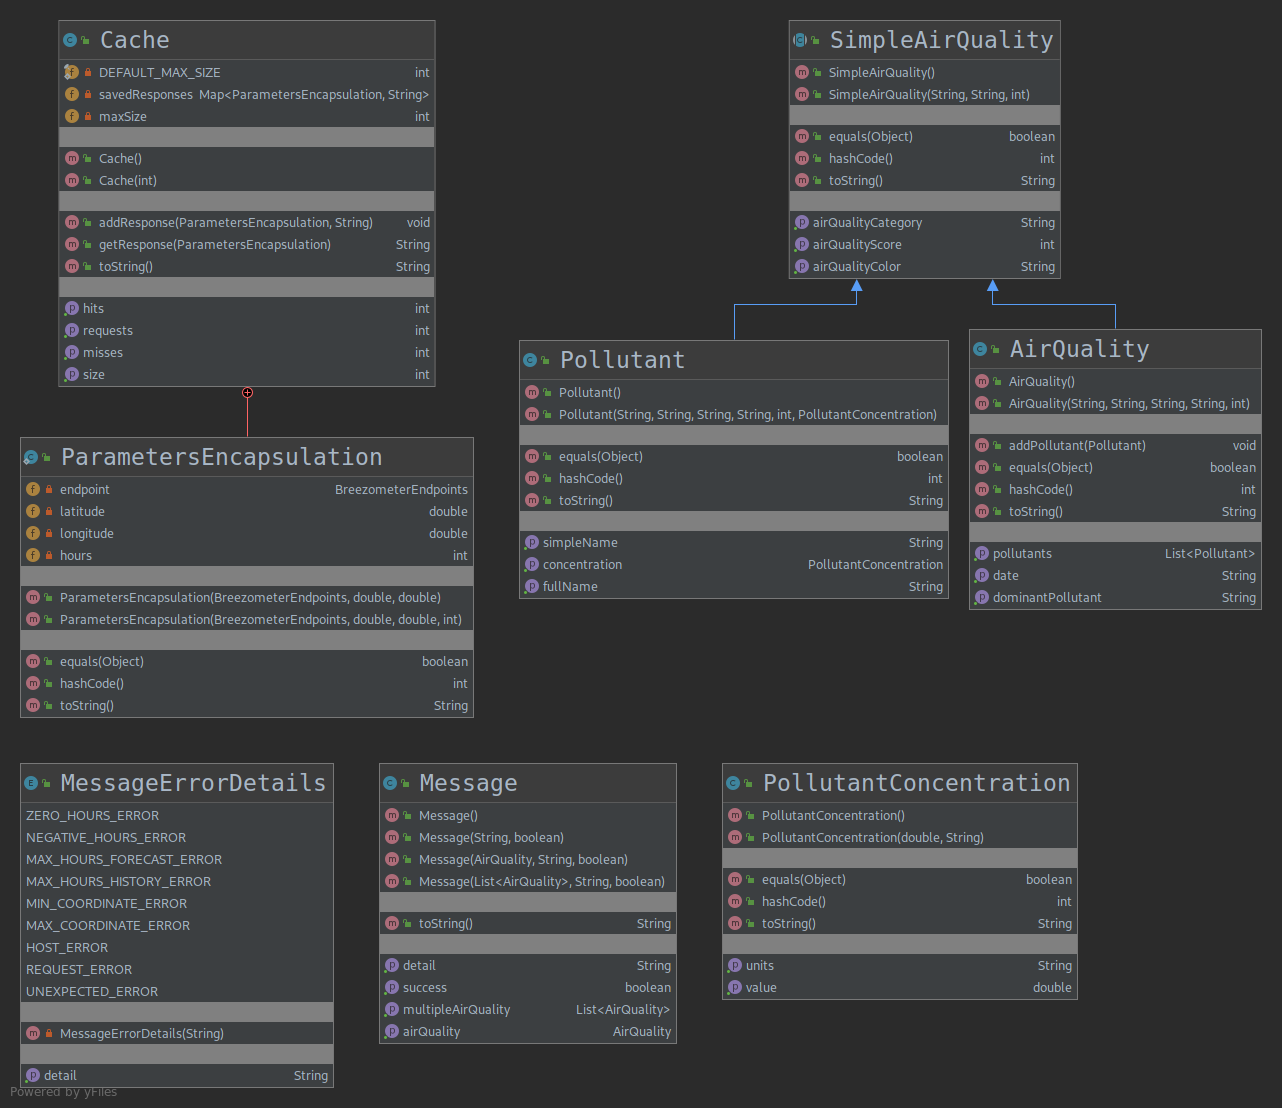
\includegraphics[width=0.90\textwidth]{images/model_diagram}
   \caption{Diagrama das classes do \textit{package \textbf{model}}.}
   \label{fig:model_diagram}
\end{figure}


\subsection{Package serializers}
De forma a poder fazer a "tradução" entre os dados recebidos do serviço externo e algumas das classes do \textit{model}, foram criados alguns \textit{deserializers} para esse efeito, como é possível verificar no diagrama da figura \ref{fig:serializers_diagram}. Para isso, foi usada a livraria \textit{Jackson}.
\begin{figure}[h]
   \centering
   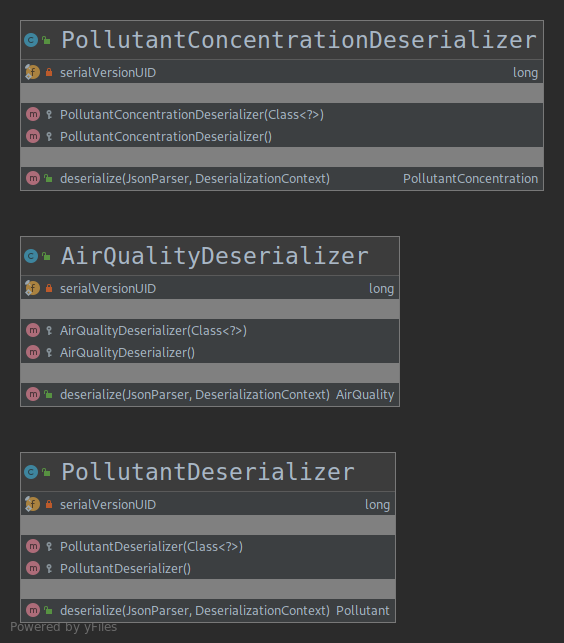
\includegraphics[width=0.90\textwidth]{images/serializers_diagram}
   \caption{Diagrama das classes do \textit{package \textbf{serializers}}.}
   \label{fig:serializers_diagram}
\end{figure}


\subsection{Package service}
De maneira a obter os dados necessários sobre a qualidade do ar, foi necessário criar um elo de ligação entre o \textit{back-end} criado e o serviço externo usado (\textit{BreezoMeter}), pelo que neste \textit{package} se encontram as classes que o permitem fazer. Quando a \textit{API} recebe um determinado pedido (excluindo o das estatísticas da cache), o método da classe \textbf{\textit{ConditionsController}} responsável por tratar do pedido "chama" o método \textit{requestApi} da classe \textbf{\textit{ConditionsController}} deste \textit{package} com o respetivo pedido, sendo que esta ultima faz um pedido ao serviço externo usando a classe \textbf{\textit{HttpBasic}} (disponibilizada pelo professor da disciplina numa das aulas práticas). A resposta do serviço externo é de seguida processada pelos \textit{deserializers} já descritos anteriormente e o objeto ou lista de objetos da classe \textbf{\textit{AirQuality}} são retornados ao método do \textit{controller} que tinha feito o pedido, encapsulados sob a forma dum objeto da classe \textbf{\textit{Message}}. Na figura \ref{fig:service_diagram} é possível encontrar a estrutura interna das classes deste \textit{package}.

\begin{figure}[h]
   \centering
   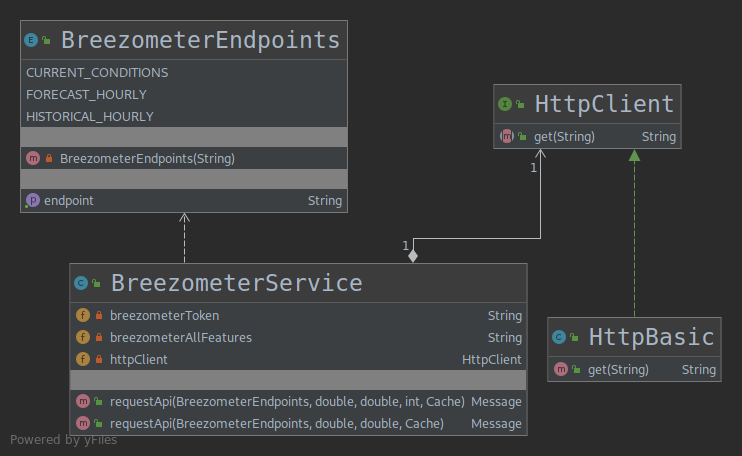
\includegraphics[width=0.90\textwidth]{images/service_diagram}
   \caption{Diagrama das classes do \textit{package \textbf{service}}.}
   \label{fig:service_diagram}
\end{figure}


\section{API para desenvolvedores}
Como já explicado múltiplas vezes ao longo deste relatório, o serviço criado permite obter informações sobre a qualidade do ar presente, passada ou futura, sendo que para isso utiliza um serviço externo para obter as informações necessárias. Assim, a \textit{API} criada possui 4 \textit{endpoints}:

\begin{itemize}
   \item \textbf{\textit{/current}}:
      \begin{itemize}
         \item Permite obter a qualidade do ar atual.
         \item Parâmetros:
            \begin{itemize}
               \item \textbf{\textit{lat}}: número decimal representante da latitude do lugar pretendido.
               \item \textbf{\textit{lon}}: número decimal representante da longitude do lugar pretendido.
            \end{itemize}
      \end{itemize}
   \item \textbf{\textit{/forecast}}:
      \begin{itemize}
         \item Permite obter a previsão da qualidade do ar até 95 horas futuras.
         \item Parâmetros:
            \begin{itemize}
               \item \textbf{\textit{lat}}: número decimal representante da latitude do lugar pretendido.
               \item \textbf{\textit{lon}}: número decimal representante da longitude do lugar pretendido.
               \item \textbf{\textit{hours}}: número inteiro representante da número de horas pretendidas.
            \end{itemize}
      \end{itemize}
   \item \textbf{\textit{/history}}:
      \begin{itemize}
         \item Permite obter o histórico da qualidade do ar até 168 horas passadas.
         \item Parâmetros:
            \begin{itemize}
               \item \textbf{\textit{lat}}: número decimal representante da latitude do lugar pretendido.
               \item \textbf{\textit{lon}}: número decimal representante da longitude do lugar pretendido.
               \item \textbf{\textit{hours}}: número inteiro representante da número de horas pretendidas.
            \end{itemize}
      \end{itemize}
   \item \textbf{\textit{/cache}}:
      \begin{itemize}
         \item Permite obter as estatísticas da cache usada (\textit{requests}, \textit{hits}, \textit{misses} e \textit{size}).
      \end{itemize}
\end{itemize}

Para informação mais detalhada sobre cada endpoint, pode ser acedida a página \url{http://localhost:8080/swagger-ui.html#/} (se a \textit{API} for iniciada em \textbf{\textit{localhost}} e na porta \textbf{8080}).
